%-------------------------------------------------------------------------------
% File: database.tex
%       Part of StockSim project documentation.
%       See main.tex for further information.
%-------------------------------------------------------------------------------
\chapter{Database}

The dataset is composd by 8236 stocks from the US stock market, along with
their general informations and historical data; the application also need to store 
users' and admins' credential, personal informationof users, composition and details of
each user's porfolio.
We decided to use a column database for the storage of historical data; those 
informations represent around the 99\%\ of our dataset and they are going to grow very fast
during time; aggregation and financial analytics on these volumes of data will perform
better in a colum database where data storage is design to optimize this type of operations;
We decided to store every other information in a document database, in order to exploit the
schemaless property for save memory; information frequently needed toghether will be stored 
in the same document and indexes are created to speedup linking beetween documents; 


\section{Dataset}
The initial set of data it's been taken from the web, thanks to www.nasdaqtrader.com
and finance.yahoo.com, using python scripts with pandas, yfinmace and json as support
libraries.
\subsection{NasdaqTrader}
The Nasdaq Stock Market (Nasdaq) is the largest U.S. equities exchange venue by volume. 
https://www.nasdaqtrader.com/ \\
We choose to take our set of stocks from the Nasdaq index, because it's very popular and
include a large number of stock, representative of differenteconomy sector. This will allow 
users to interact with big and famous comopanies stocks (like Google, Apple, Tesla...), but also
to try smaller companies and/or minor sectors investemts. 
NasdaqTrader provides us a stocks'symbols' list of all the stocks entered in the nasdaq index
from 1970 till now;
\subsection{Yahoo! Finance}
"Yahoo Finance provides free stock quotes, up-to-date news, portfolio management resources, 
international market data, social interaction and mortgage rates that help you manage your 
financial life." https://finance.yahoo.com/ \\
Yahoo Finance is a service, been part of the yahoo network, that provide a lot of information
about stocks and companies; they are frequantly updated, relible and good organized.\\
We decided to use this service to retrive the starting dataset of stocks; we extract only 
the fields that we needed, and parse into a JSON file. In this way 
is possible to rebuild from scratch this dataset into mongoDB with few commands (including
mongoimport).
With Yahoo Finance is also possible to retrive historical data of market values for every 
stocks. Using this service it's been possible to build a dataset of all the market values of
each stocks coming from NasdaqTrader; values are collected daily, and we decided to take all 
the values from 2010 to 2020; this dataset (around 1.43 GB) it's been parsed to CVS files and
than imported into a Cassandra Cluster. Thanks to the Yahoo Finance service, it's possible
to update every day the databse with the last session results. It's also possible to add a new
stock to the dataset, coming from every market exchange of every country.\\
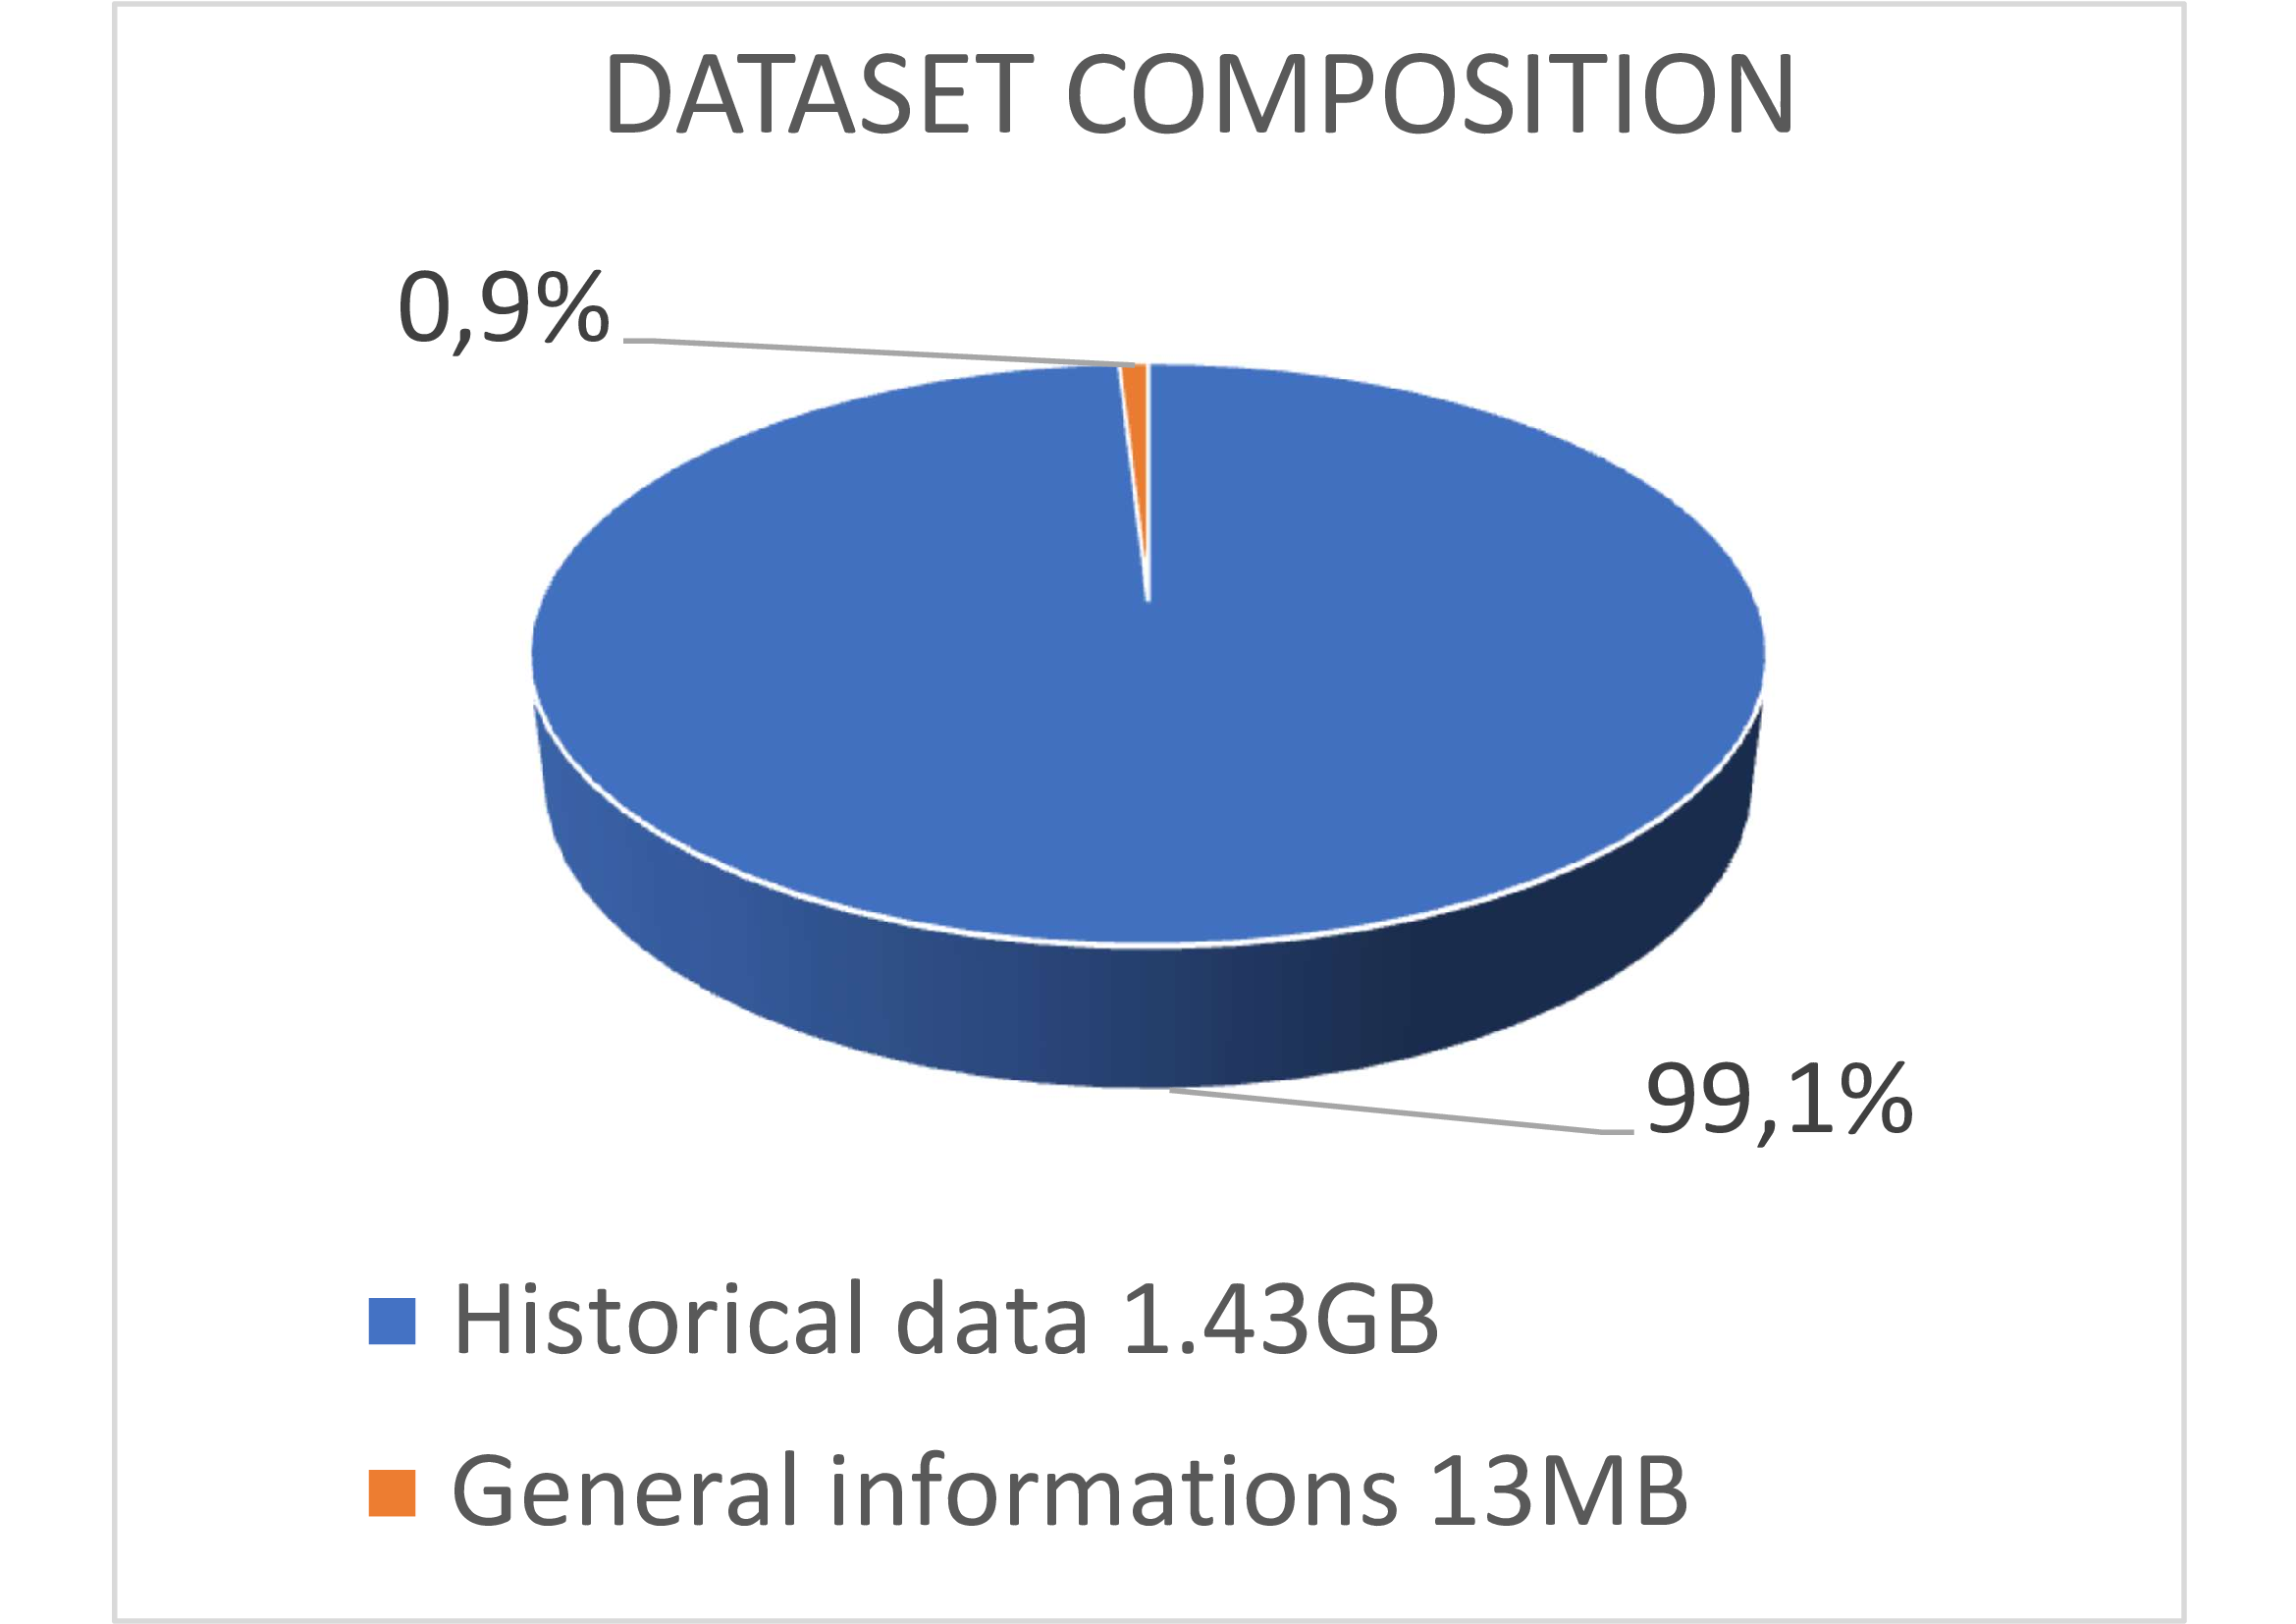
\includegraphics[scale=0.12]{img/dataset_comp.png}\\


\section{MongoDB}
"MongoDB is a general purpose, document-based, distributed database build
for modern application developers and for the cloud era." Taken from www.mongodb.com.\\
MongoDB is a very famous document database with a great support for cloud operations, witch 
will improve the avaliability of our application. It also suport a lot of analytics functions
and the creation of custom indexes in order to speedup read operations.
In order to orgnize data ina a meaningfull and memery-optimal way, we opted for this structure:

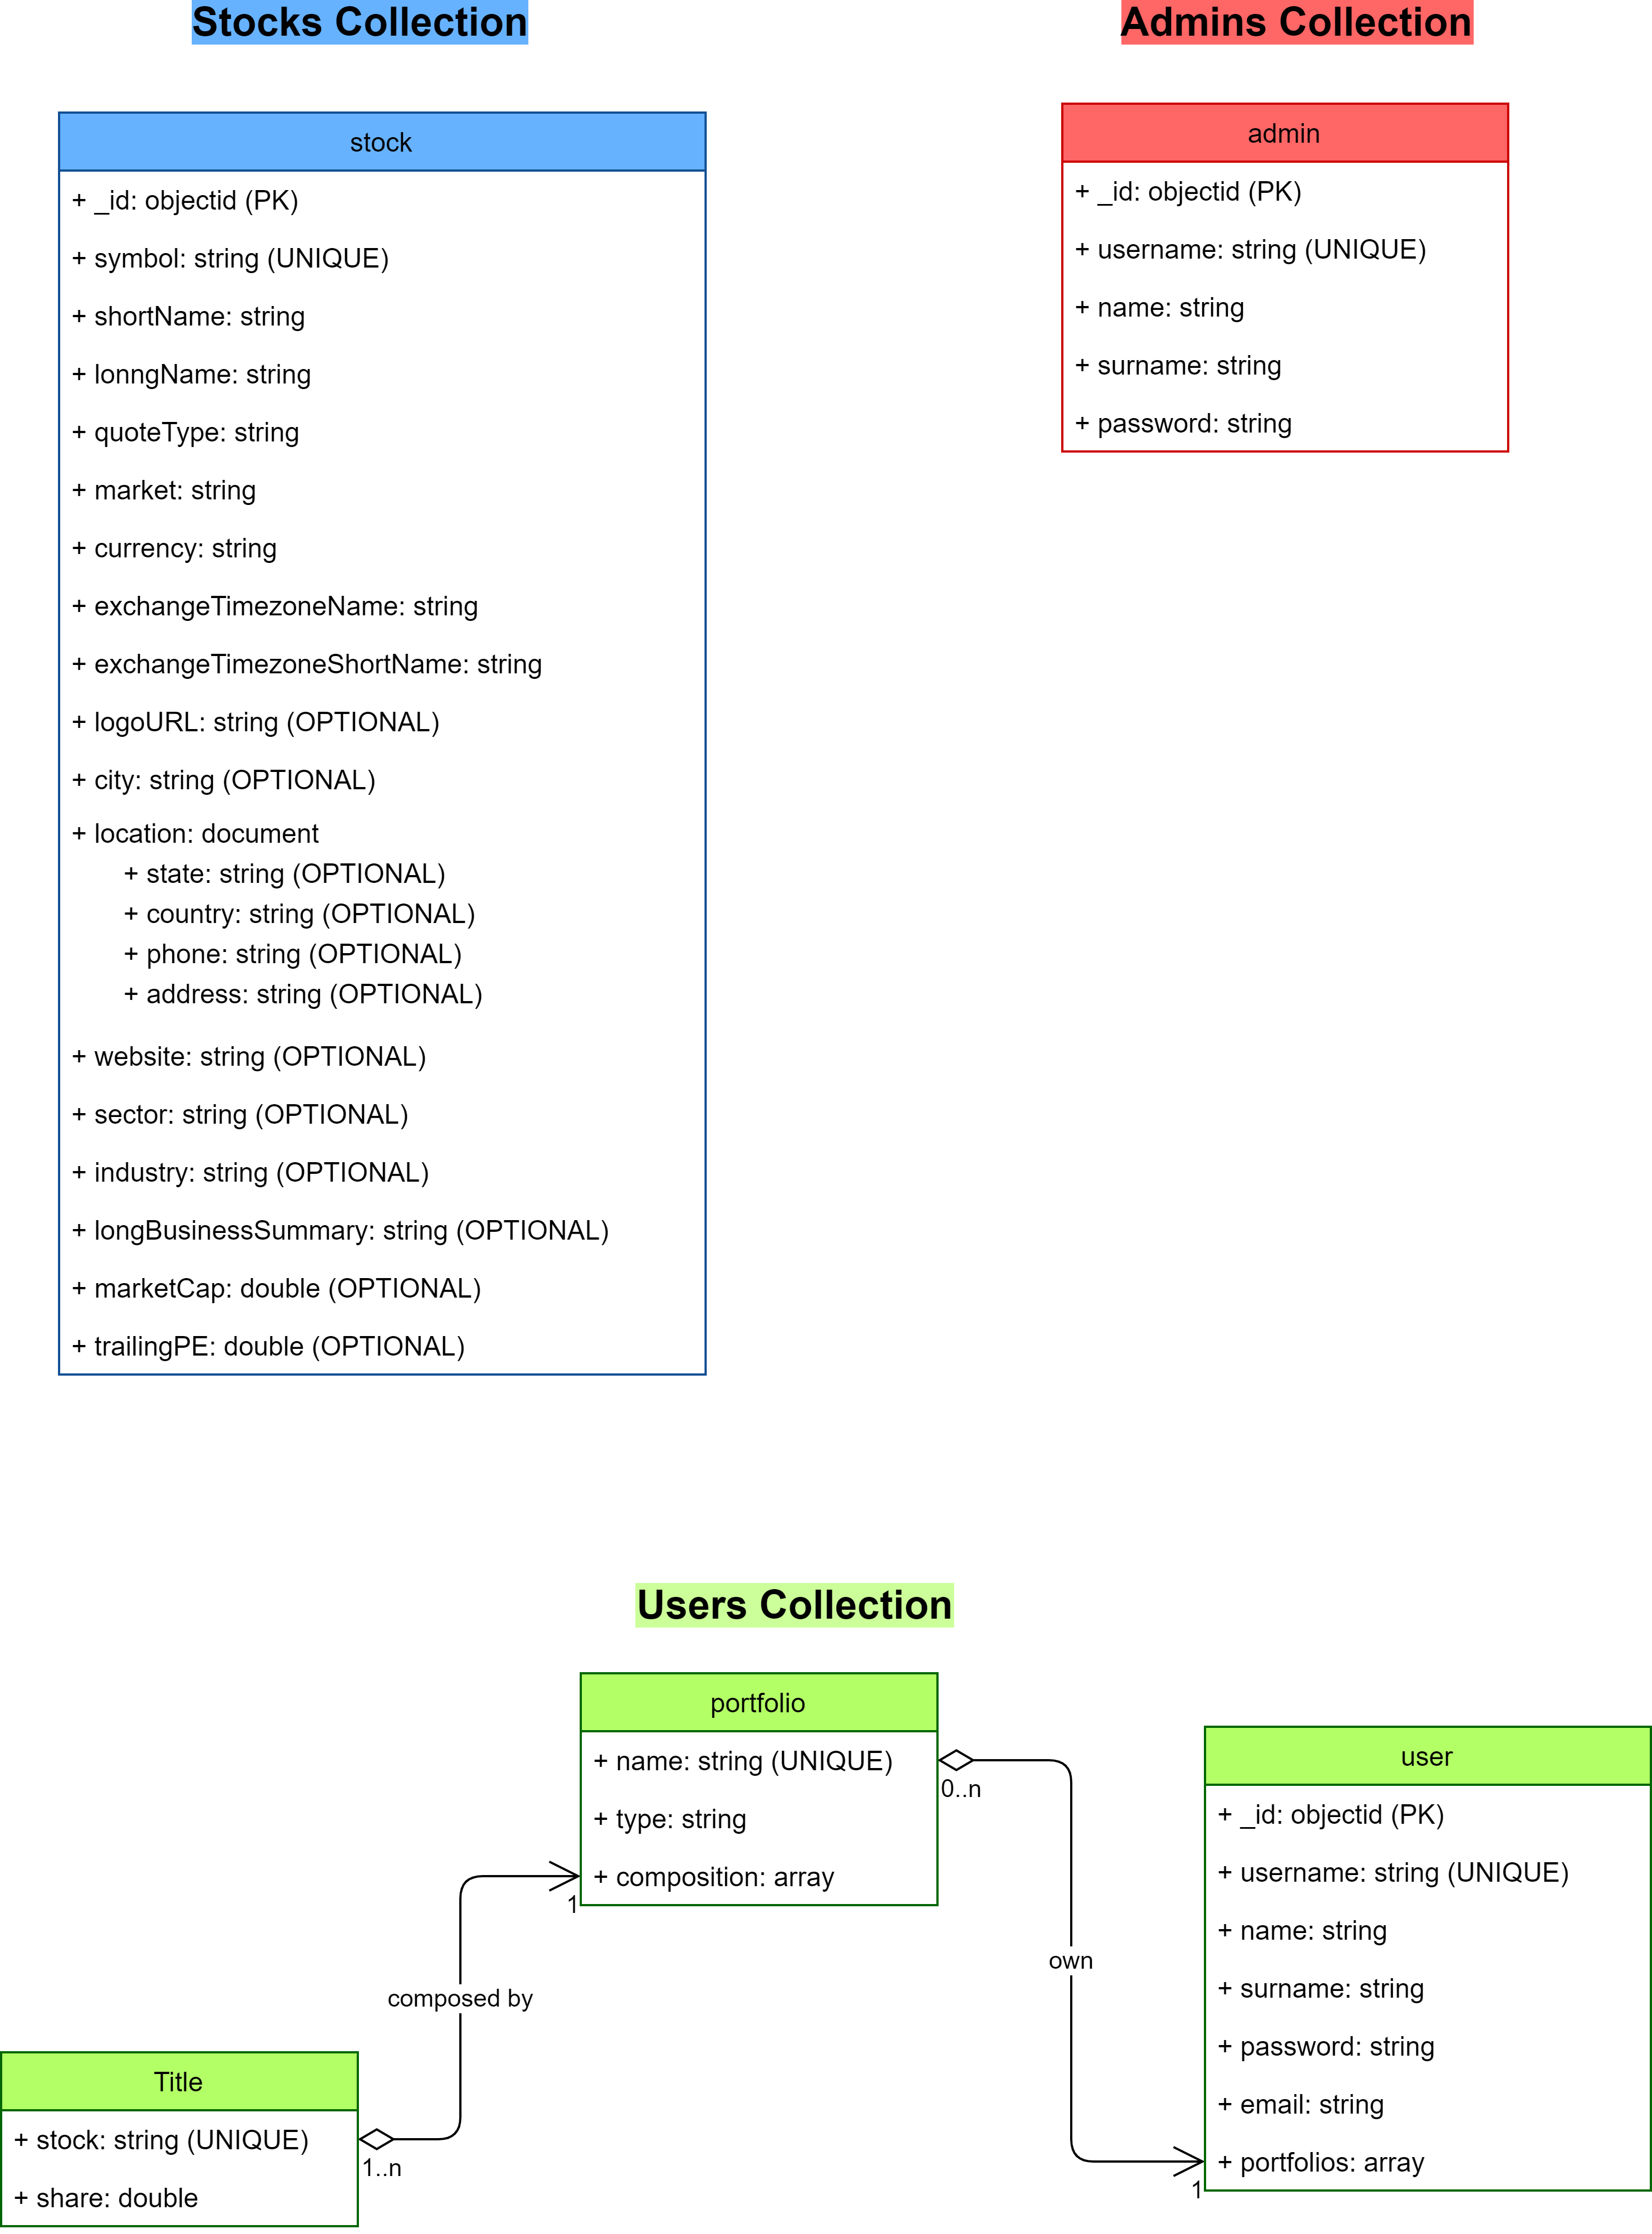
\includegraphics[scale=0.17]{img/mongoDB_schema.png}\\

This scheme is composed by 3 collections: \textbf{stocks}, \textbf{users}, \textbf{admins};
\begin{itemize}
    \item
The stocks collection contains one document for each stock; inside this document are stored 
all the general information about the stock, wich is identified by the attribute SYMBOL;
some basic information are always presents, while others are missing for some stocks; we decided 
to keep these last type of informations where possible, exploiting the schemaless property of
the documentat databse;
    \item
The users collection contains one docuemt for each user regitered on the application; for every
user login credentials are stored, along with few personal information; for every user is 
also stored an array of documents named PORFOLIOS: this array contains the porfolios of the user.
Each portfolio has a scheme, witch include an array of TITLEs, named COMPOSITION, witch represent
the settlement of the portfolio itsef. This nested structure it's been preferred from splittin
data in different collections, because all the information of a user, including his portfolios, 
are frequently needed toghether; on the other hand, there aren't such operations that involve
porfolios owneds by different users.
    \item 
The admins collection contains the admins login credentials toghether with few personal
informations about them; we decided to crerate a separated collection for administators 
to improve the security of the administration features: in this way is impossible to inject
administration privileges throw the login command.
\end{itemize}
\subsection{Aggregations}
One of the main features of own application is the possibility to choose some stocks from
the market and combine them in to a portfolio. When a user is looking for a stock, he want to
know statistic about \textbf{industies} and \textbf{sectors}, along with classification by 
\textbf{level of capitalization} and  \textbf{PE ratio}; in ordewr to do so, we will provide
these aggregation pipelines:
\begin{itemize}
    \item the total market capitalization of each sector
    \item the total market capitalization of each industry
    \item the total market capitalization of stocks coming from the same country
    \item the avarage PE ratio of stocks working in the same sectors
    \item the avarage PE ratio of stocks working in the same industry
    \item the avarage PE ratio of stocks coming from the same country
    \item the avarage PE ratio of stocks beeing in a specific range of market capitalization
\end{itemize}
We provide here an example of an aggregation mongo query:
\begin{lstlisting}[basicstyle=\footnotesize,language=Java,numbers=left,
    numberstyle=\footnotesize,numbersep=4pt,frame=single]
    /**
    * Aggregates data with filtering and grouping by an attribute, can compute
    * sum, avg ecc.
    *
    * @param collection the collection where to perform the operation;
    * @param filter filter to be used to find the documents.
    * @param groupField the filed used to group the aggregation
    * @param aggregator the aggregator function and field
    *
    * @return iterable object containing the result of the aggregation.
    */
   public AggregateIterable<Document> aggregate(final Bson filter, final String groupField, final BsonField aggregator, final MongoCollection<Document> collection) {
       Bson match = Aggregates.match(filter);
       return  collection.aggregate(
               Arrays.asList(match, Aggregates.group("$"+groupField, aggregator)));
   }
\end{lstlisting}
\begin{lstlisting}[basicstyle=\footnotesize,language=Java,numbers=left,
    numberstyle=\footnotesize,numbersep=4pt,frame=single]
    MongoCollection<Document> collection1 = 
        dbManager.getCollection(
            StocksimCollection.STOCKS.getCollectionName()
        );
    // aggregate examples
    final Bson equity= eq("quoteType", "EQUITY"); //filter(s)
    // name of the field projected, field to accumulate
    // type of accumulation (sum, avg...)
    final BsonField marketCapAccumulator=Accumulators.sum("totalCap","$marketCap");
    AggregateIterable<Document> aggregateList =
                                        // grouping attribute
            dbManager.aggregate(equity, "sector", marketCapAccumulator, collection1);
    for (Document document : aggregateList) {
        System.out.println(document);
    }
    // avg example with nested attribute
    final BsonField PEAccumulator=Accumulators.avg("avgPE","$trailingPE");
    aggregateList =
            dbManager.aggregate(equity, "location.country",
                    PEAccumulator, collection1);
    for (Document document : aggregateList) {
        System.out.println(document);
    }
\end{lstlisting}
\subsection{Indexes}
In order to speeup read operation in the document database, 
we decided to introduce some custom indexes:
\begin{itemize}
    \item a REGULAR and UNIQUE index on the attribute \textbf{symbol} in the collection stocks;
    \item a REGULAR index on the attribute \textbf{marketCAP} in the collection stocks;
    \item a REGULAR index on the attribute \textbf{trailingPE} in the collection stocks;
    \item a REGULAR index on the attribute \textbf{sector} in the collection stocks;
    \item a REGULAR index on the attribute \textbf{industry} in the collection stocks;
    \item a REGULAR index on the attribute \textbf{country} in the collection stocks;
    \item a REGULAR and UNIQUE index on the attribute \textbf{username} in the collection users;
\end{itemize}
We provide some statistic that endorse our idexes choises\\

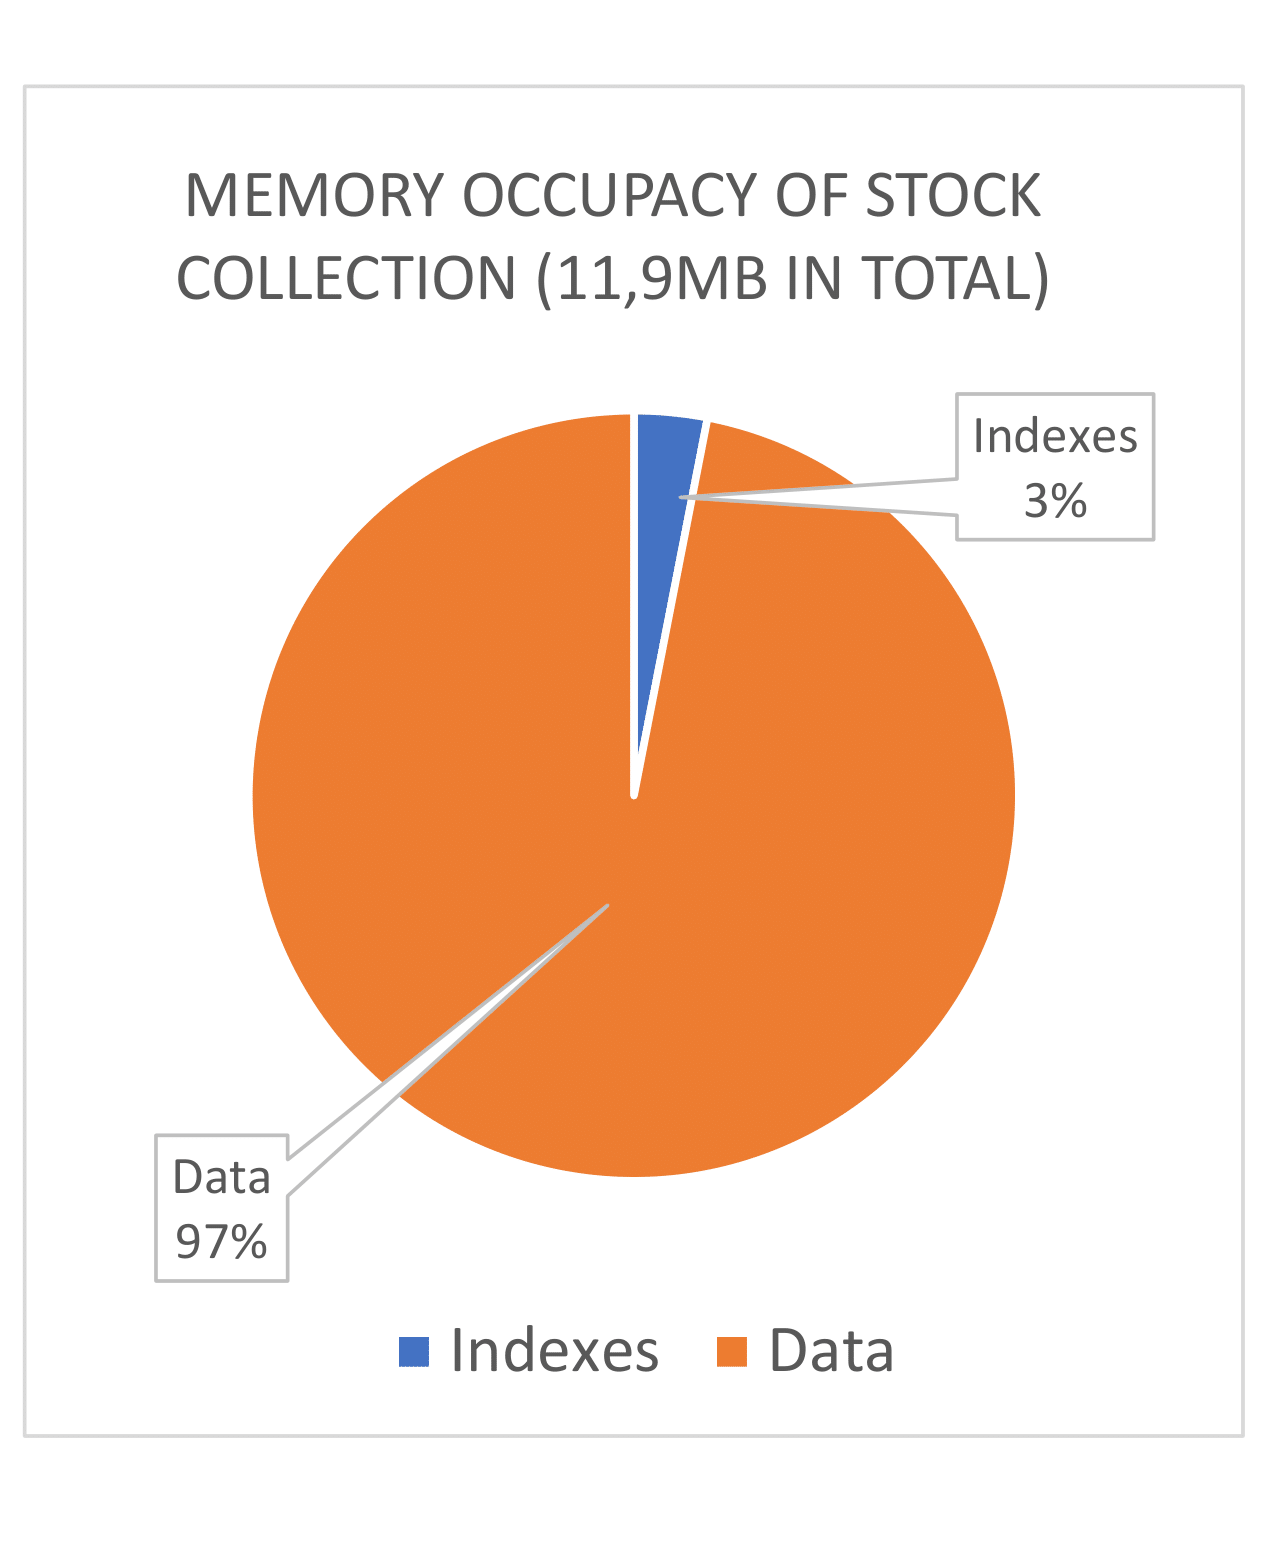
\includegraphics[scale=0.11]{img/memory_mongo.png}
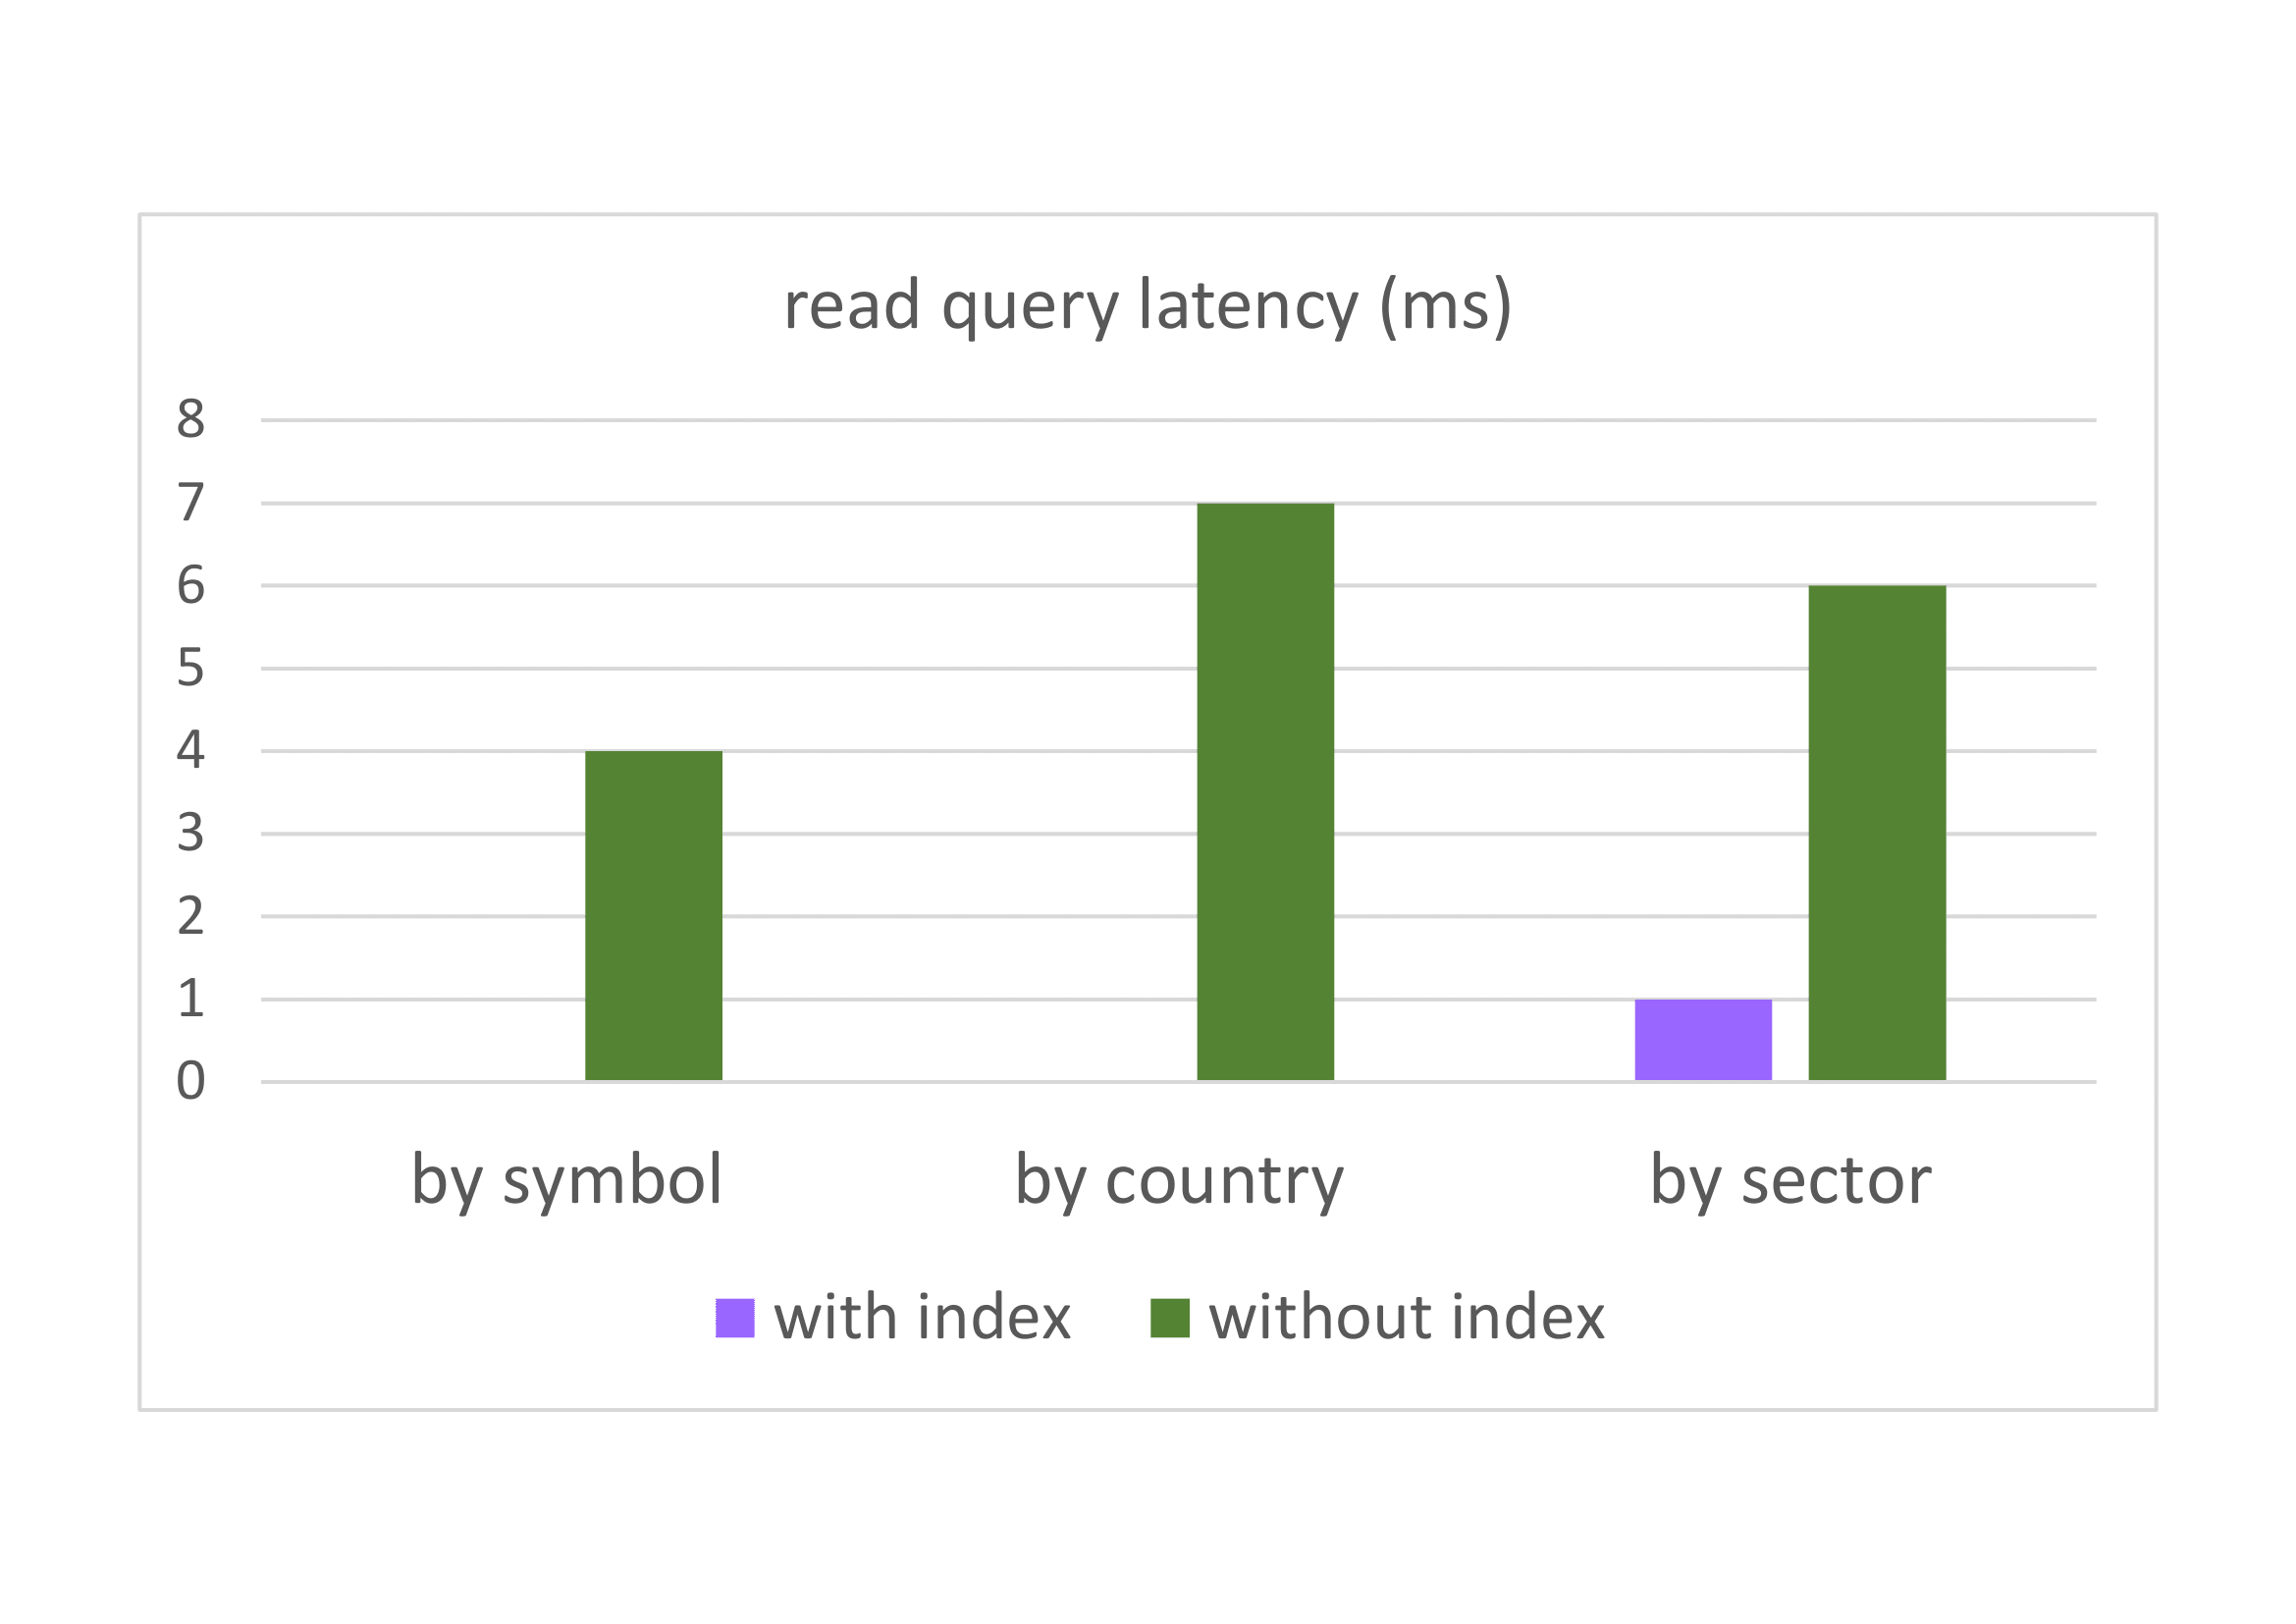
\includegraphics[scale=0.11]{img/latency_mongo.png}\\

Analog results can be found about the username index in the users collection.

\section{Apache Cassandra}
"The Apache Cassandra database is the right choice when you need scalability and high 
availability without compromising performance. Linear scalability and proven fault-tolerance 
on commodity hardware or cloud infrastructure make it the perfect platform for mission-critical 
data. Cassandra's support for replicating across multiple datacenters is best-in-class, 
providing lower latency for your users and the peace of mind of knowing that you can survive
regional outages." www.cassandra.apache.org\\
Apache Cassandra is a database designed for high scalability and availability; it's 
capable to handle a huge amount of data and manage it in a decentralized architecture
across multiple nodes. It's build to be write optimized, but with right indexes choises
also read latency can be improved; tables schemes and analytics functions can be customized.
This is the scheme of our Cassandra databse:\\
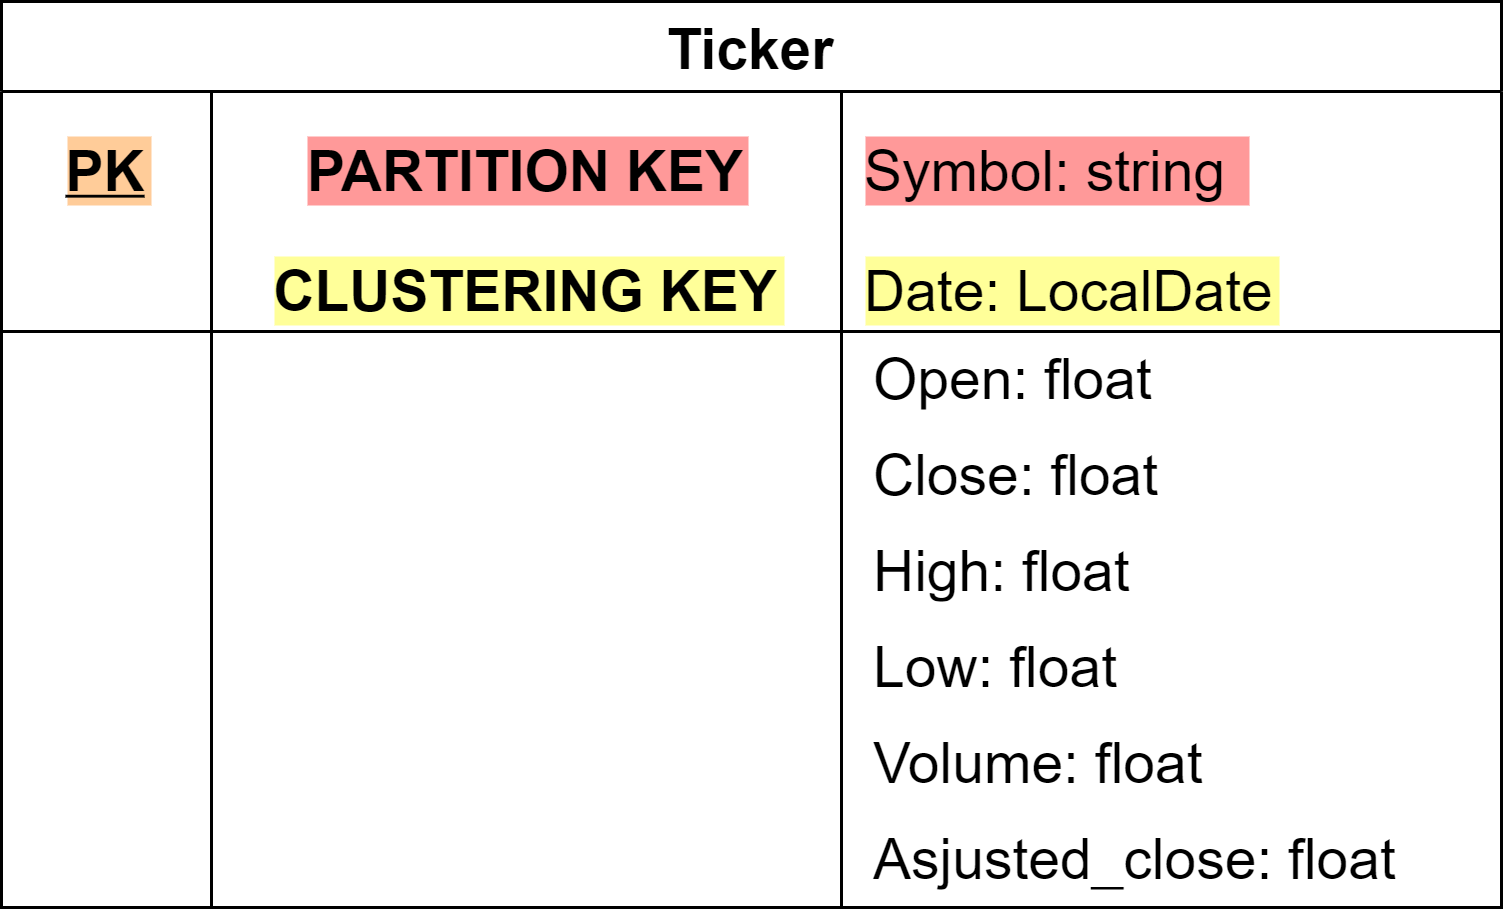
\includegraphics[scale=0.2]{img/cassandraDB_scheme.png}\\

\subsection{Aggregations}
In order to provide snaphots and statistics of stocks and portfolios trends oevr time,
we explit the customization functionalities of Cassandra; a custom aggaregation it's been 
created, specifically to provide aggegate values of more than one day, for a given
perdiod of time; this allow us to obtain different granularity for stock market data,
computed on server side; this will not over overwelm the server, because the aggregator will
execute, for each row, beetween a memory access and the following. This will reduce by a lot
the data to be transitted from the node to the client, saving bandwith and time.  \\

\begin{lstlisting}[basicstyle=\footnotesize,language=SQL,numbers=left,
    numberstyle=\footnotesize,numbersep=4pt,frame=single]

    /* State function to be executed for every row*/
    CREATE OR REPLACE FUNCTION PeriodStateParam ( 

    /* the state, containing the aggregation result till this row */
        state map<date,frozen<map<text, float>>>,
    /*  the parameter ndays indicate the duration 
    *   of the period aggregation, in days          */
        ndays int, data date,  
        open float,  close float , high float,  low float, 
        volume float ,  adj_close float)
    CALLED ON NULL INPUT 
    RETURNS map<date,frozen<map<text, float>>> 
    LANGUAGE java AS '
    if (data != null) { 
        int d=0;
        Map<String, Float> statemap=null;
       
        for(d=1; d<ndays;){
            if((statemap=state.get(
                    data.add(Calendar.DAY_OF_MONTH,d)
                ))!=null)
                break;
            d++;
        }
        if(d==ndays){
            statemap=new HashMap<String, Float>();
            statemap.put("open", open);
            statemap.put("close", close);
            statemap.put("high", high);
            statemap.put("low", low);
            statemap.put("volume", volume);
            statemap.put("adj_close", adj_close);
            state.put(data,statemap);
        }
        else{
                if(high>statemap.get("high"))
                    statemap.replace("high", high);
                if(low<statemap.get("low"))
                    statemap.replace("low", low); 
                statemap.replace("volume",statemap.get("volume")+ volume);
                statemap.replace("open",open);
                state.replace(data, statemap); 
        }
    } 
    return state;'
     ;
    
    /*  aggregate declartation
    *   this aggregation geenrate a map data structure (JSON like):
    *   the key is the end date of each period of nday days, 
    *   and the value is another map containing the aggregate 
    *   values of the period as:
    *        the open of the first day
    *        the close and adjusted close of the last day
    *        the maximun of the highs
    *        the minimum of the lows
    *        the sum of the volumes
    */
    CREATE OR REPLACE AGGREGATE PeriodParam 
        ( int, date,float, float,float, float,float, float ) 
    SFUNC PeriodStateParam
    STYPE map<date,frozen<map<text, float>>>
    INITCOND {}; /* no initial condition is necessary */
    
    /* example of usage, it can be used also with grouping by symbol */
    select PeriodParam(
        20, date, open, close, high, low, volume, adj_close)
        as Period from tickers where 
        date<'2020-12-1' and date>'2020-6-10' 
        and symbol='TSLA';
    
\end{lstlisting}

\subsection{Indexes}
\begin{itemize}
    \item 
The PARTITIO KEY index is part of the PRIMARY KEY and it's used to shard the dataset across
the nodes. This index is build on the string symbol, unique for each stock;
    \item
the CLUSTERING KEY it's also part of the PRIMARY KEY, and it's used to mantain rows 
chronologic orde. This index is build on the attribute date;
\end{itemize}
\section{Sharding and Replicas}
The MongoDB cluster and the Cassandra cluster are deployed on 3 vitual machines provided
by the University of Pisa; 
Our architecture is oriented to the availability of the service, and build for the maximum
scalability and decentralization.
\begin{itemize}
    \item 
The casandra cluster is build among all 3 nodes, and data are sharded by the ticker symbol;
in this way every node store 1/3 of the main dataset, and aggregation functions are computed
on records that stay in the same node; each node also store a backup of the data
assigned to another node, give us a replicazion factor of 2. There are 2 seed nodes,
wich are responsible for the cluster: the cluster is online as long as one of them keep
working. This is indeed a minor issue, because in any case, with only ne node, the dataset 
would by incomplete. The decentralized behavior of Cassabdra ensure than
even if all the node go offline, the cluster return available as soon as one seed server go back
online. 
    \item
The mongoDB cluster is also build among all 3 virtual machines, and the service is replicated;
an initial primary server is elected, then another one will take it's place if it goes down. 
The cluster is available as long as one server is working, and incoming traffic could be balanced
with the "nearest" preference on client connection; in this way the client would connect to the
server with the lowest ping time.

\end{itemize}
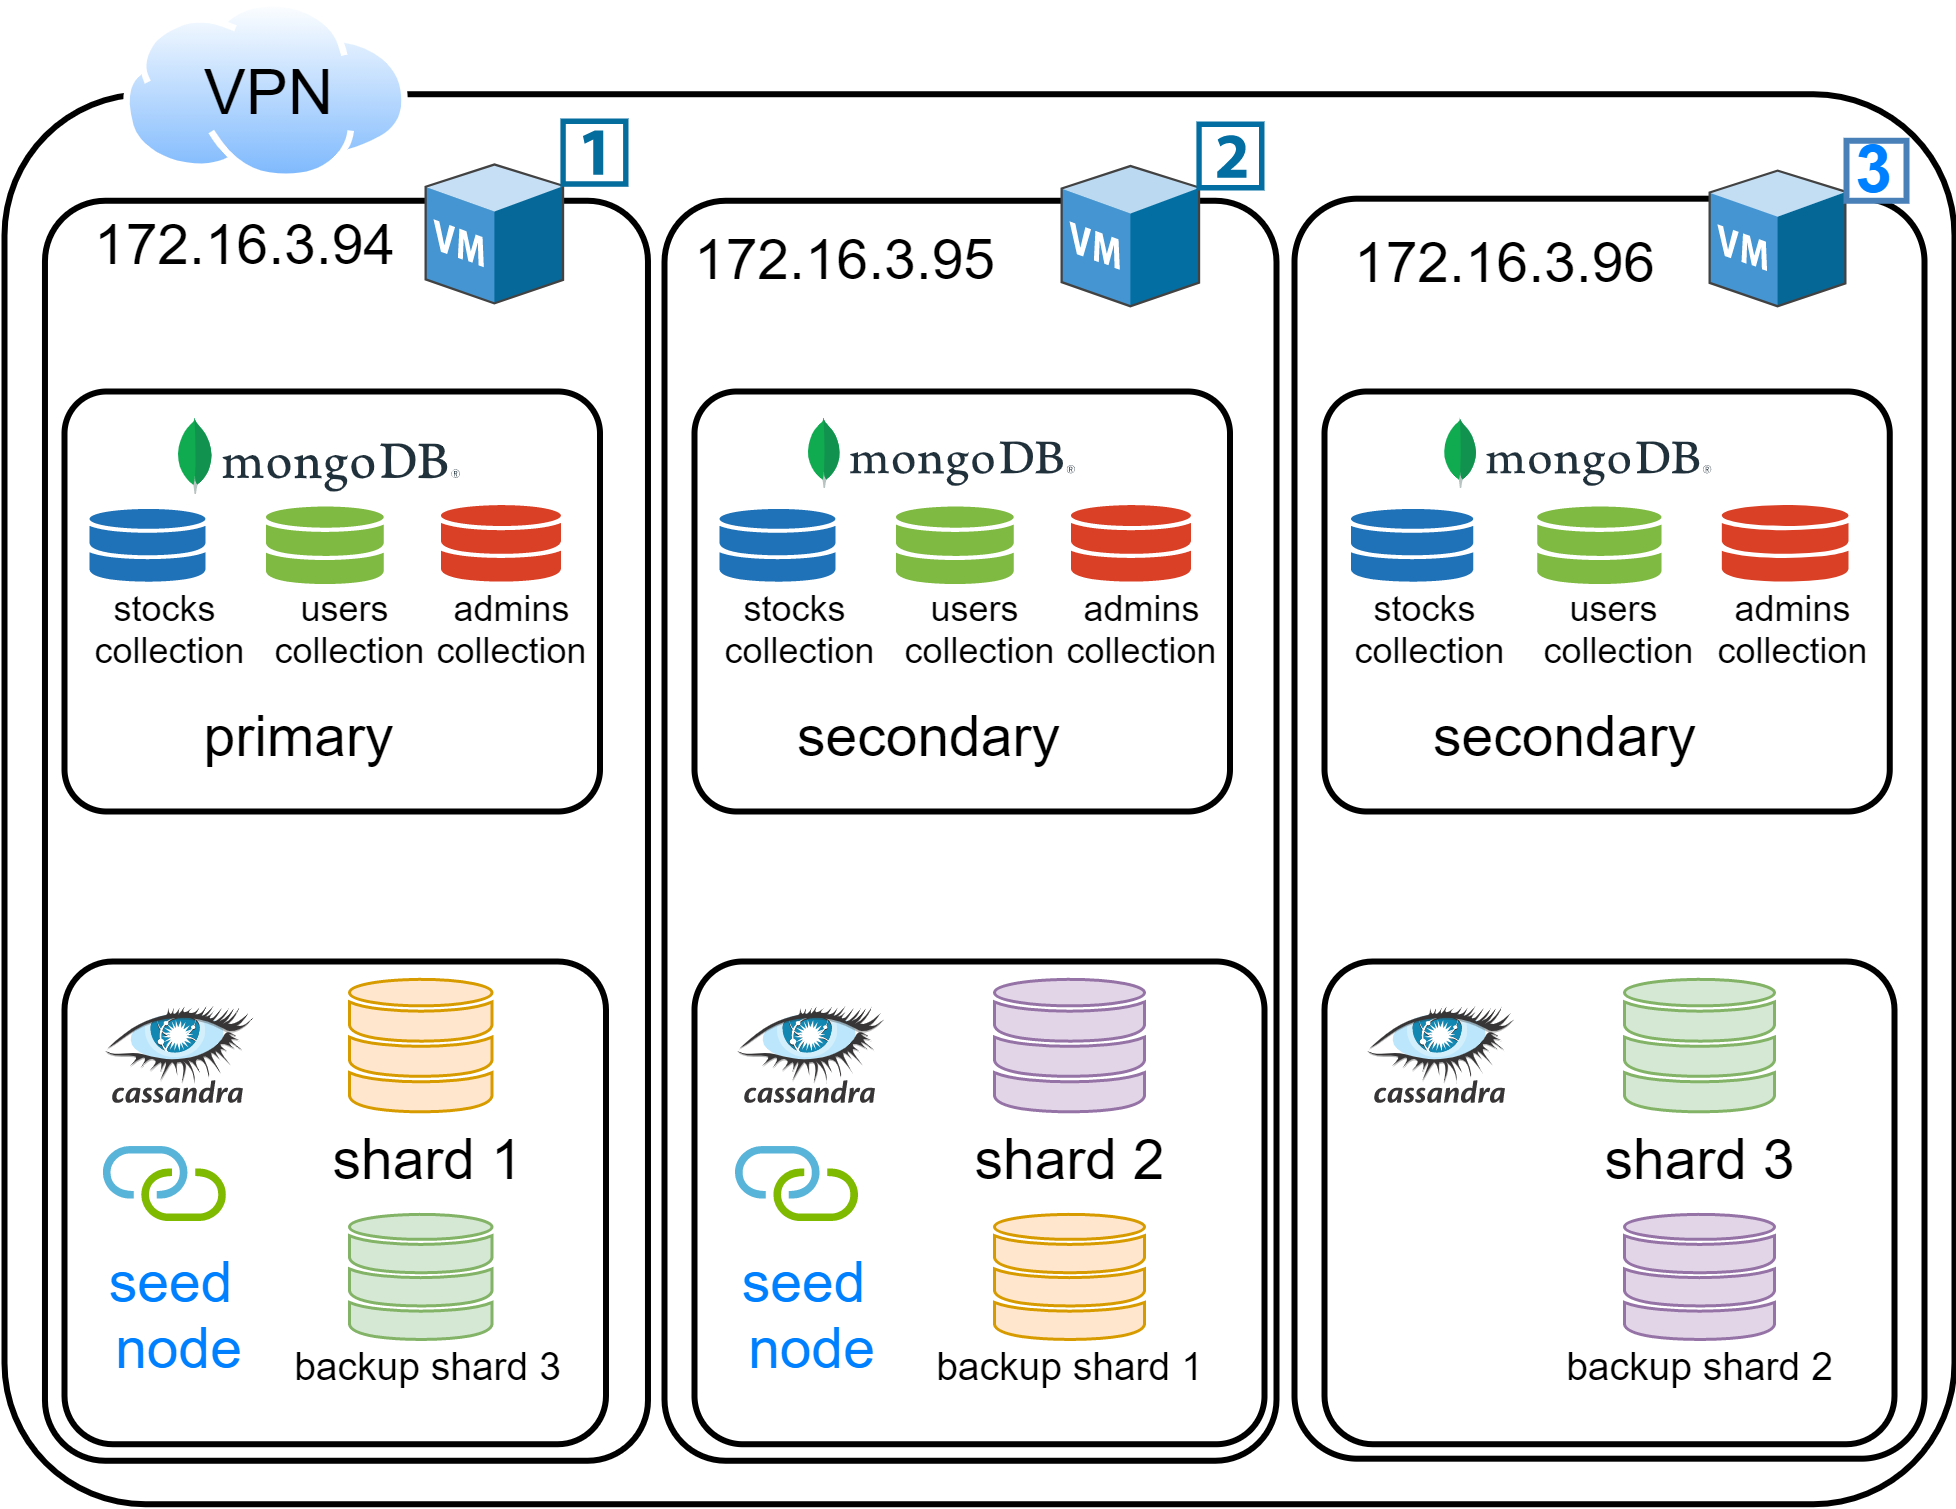
\includegraphics[scale=0.2]{img/cluster_diagram.png}\\
\section{Apache Cassandra vs MongoDB}
